\chapter{Fuentes de datos}

En este capítulo se describen las fuentes de datos utilizadas en el proyecto. Se trabaja con el conjunto MIMIC-IV tanto en su versión demo (aprox. 100 pacientes, de acceso abierto) como en su versión completa (acceso restringido). Cuando procede, se diferencian ambas para contextualizar tamaño y cobertura.

\section{Estructura del dataset}

%\subsubsection{Entendiendo los datos}

MIMIC-IV recoge sus datos de distintas fuentes, y realiza todo un complejo proceso de conversión, transformación, anonimización, clasificación y corrección de los datos hasta obtener el resultado final \cite{MIMICIV_paper}.

\begin{figure}[H]
    \centering
    \fbox{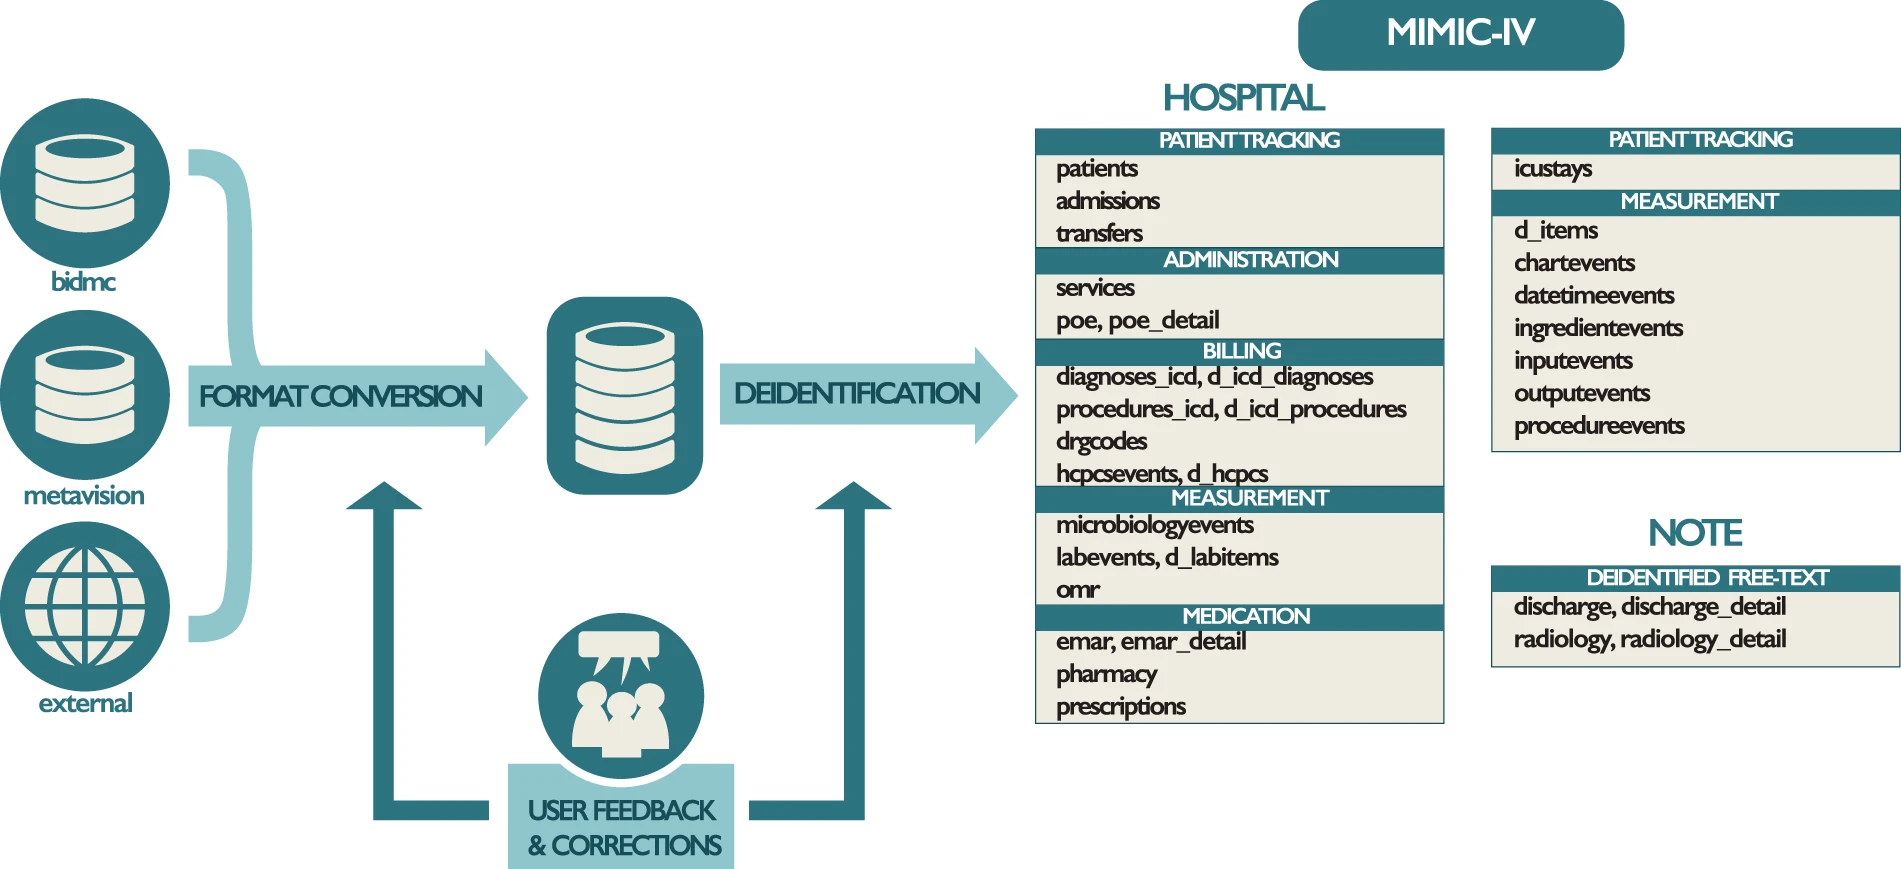
\includegraphics[width=0.95\textwidth]{imagenes/desarrolloMIMIC-IV.png}}
    %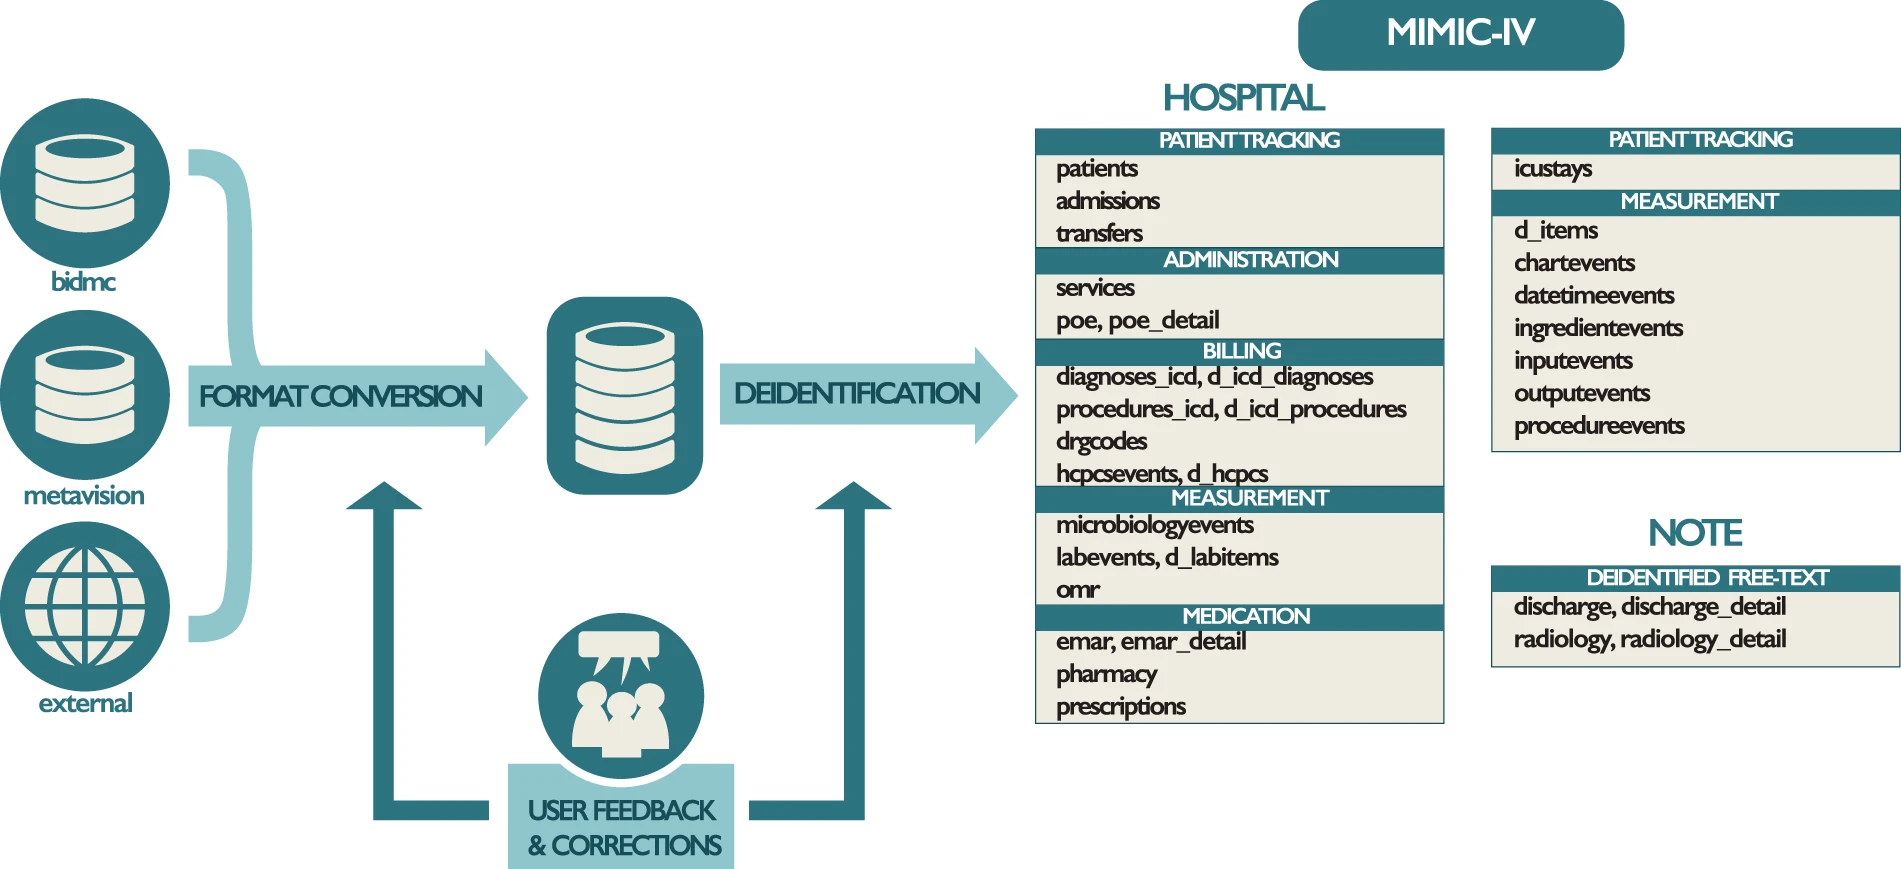
\includegraphics[width=0.95\textwidth]{imagenes/desarrolloMIMIC-IV.png}
    \caption{Resumen del proceso de desarrollo de MIMIC-IV. \cite{MIMICIV_paper}}
    \label{fig:desarrollo_mimiciv}
\end{figure}


Los datos, tal y como se han recibido, se estructuran módulos o ``carpetas", cada uno compuesto por diferentes tablas o ``archivos" que recogen distintos aspectos de la estancia hospitalaria del paciente. A continuación se resumen los dos módulos que se utilizan en el proyecto y sus tablas más relevantes:

\begin{itemize}
    \item \textbf{hosp}: Información hospitalaria general procedente del sistema de historia clínica electrónica. Incluye:
    \begin{itemize}
        \item \texttt{patients}: datos demográficos como sexo, edad y fecha de fallecimiento.
        \item \texttt{admissions}: detalles de los ingresos hospitalarios.
        \item \texttt{transfers}: movimientos de los pacientes entre distintas unidades.
        \item \texttt{labevents} y \texttt{d\_labitems}: resultados de laboratorio y su descripción.
        \item \texttt{microbiologyevents}: cultivos microbiológicos.
        \item \texttt{prescriptions}, \texttt{pharmacy}, \texttt{emar}, \texttt{emar\_detail}: información sobre prescripciones y administración de medicamentos.
        \item \texttt{diagnoses\_icd}, \texttt{d\_icd\_diagnoses}: diagnósticos realizados y codificados (ICD-9/10).
        \item \texttt{procedures\_icd}, \texttt{d\_icd\_procedures}: procedimientos realizados y codificados (ICD-9/10).
        \item \texttt{hcpcsevents}, \texttt{d\_hcpcs}, \texttt{drgcodes}: información de facturación y codificación hospitalaria.
        \item \texttt{services}: servicios hospitalarios responsables del paciente.
        \item \texttt{poe}, \texttt{poe\_detail}: órdenes médicas realizadas por los profesionales.
        \item \texttt{provider}, \texttt{omr}: información sobre proveedores y registros médicos online.
    \end{itemize}
    \item \textbf{icu}: Datos recogidos específicamente durante la estancia en la UCI, provenientes del sistema clínico MetaVision. Incluye:
    \begin{itemize}
        \item \texttt{icustays}: información sobre las estancias en UCI.
        \item \texttt{chartevents}: registros detallados de constantes, procedimientos, observaciones y eventos clínicos.
        \item \texttt{inputevents}, \texttt{ingredientevents}: administración de fluidos, nutrición y medicamentos intravenosos.
        \item \texttt{outputevents}: registros de salidas del paciente (orina, drenajes, etc.).
        \item \texttt{procedureevents}: procedimientos realizados en UCI.
        \item \texttt{datetimeevents}: eventos documentados con fecha y hora.
        \item \texttt{d\_items}: diccionario de variables y conceptos registrados en los eventos.
        \item \texttt{caregiver}: identificadores de los profesionales sanitarios en UCI.
    \end{itemize}
\end{itemize}


En nuestro caso, utilizamos estos dos módulos pero hay más, como \textbf{ed} (emergency department), \textbf{cxr} (radiografías de tórax) y \textbf{note} (notas clínicas desidentificadas), que amplían la información disponible para cada paciente.

Un aspecto fundamental para trabajar con MIMIC-IV es la correcta utilización de los campos identificadores que permiten relacionar la información entre tablas y reconstruir la trayectoria clínica de cada paciente:

\begin{itemize}
    \item \texttt{subject\_id}: identificador único de paciente, presente en prácticamente todas las tablas. Permite agrupar toda la información relativa a una misma persona a lo largo de distintas estancias y episodios.
    \item \texttt{hadm\_id}: identificador único de cada ingreso hospitalario. Cada hospitalización de un paciente tiene uno distinto, lo que permite diferenciar varios ingresos de la misma persona y asociar eventos, pruebas y tratamientos concretos a cada episodio.
    \item \texttt{stay\_id} (en ICU): identifica de forma única cada estancia en la UCI, permitiendo enlazar los eventos críticos de cuidados intensivos.
    \item Otros identificadores secundarios: \texttt{specimen\_id} (muestras de laboratorio), \texttt{pharmacy\_id}, \texttt{order\_provider\_id} (profesional que ordena una prueba o medicación), \texttt{itemid} (tipo de medición o concepto registrado), entre otros.
\end{itemize}

Además de todos estos datos, se creó manualmente otro archivo \texttt{icd\_equivalencias}, el cual contiene las equivalencias entre códigos ICD-9 e ICD-10. Los códigos ICD (International Classification of Diseases) son el estándar internacional para clasificar enfermedades, diagnósticos y procedimientos médicos. Esta tabla permite unificar datos codificados en ambas versiones y aporta una clasificación jerárquica organizada en capítulos (chapters), supersecciones (super sections) y secciones (sections). Por ejemplo, el código ICD-9 ``0090'' (Infectious colitis, enteritis, and gastroenteritis) se mapea al ICD-10 ``A09'' y se clasifica dentro del capítulo ``A'' (Certain infectious and parasitic diseases), supersección ``A00-A09'' (Intestinal infectious diseases) y sección ``A09'' (Infectious gastroenteritis and colitis, unspecified). Esta estructura facilita el análisis y visualización de diagnósticos por categorías médicas.

En conclusión, toda esta estructura modular nos permite, a nivel de paciente, reconstruir de forma detallada la trayectoria clínica, desde su ingreso hasta el alta, pasando por episodios críticos, pruebas, tratamientos y evolución. A nivel global, las posibilidades son enormes, para calcular estadísticas, visualizaciones, y todo tipo de agregaciones de las que se pueda extraer conocimiento. Para más detalles sobre los datos, puede consultarse la documentación oficial de MIMIC-IV \cite{MIMICIV_docs}.

\section{Estadísticas básicas}

La Tabla~\ref{tab:estadisticas_basicas} resume el número de filas por archivo para las versiones demo y completa.

\begin{table}[H]
  \centering
  \small
  \begin{tabular}{|l|c|c|}
    \hline
    \textbf{Archivo (colección)} & \textbf{Demo filas} & \textbf{Full filas} \\
    \hline
    admissions & 275 & 546\,028 \\
    d\_hcpcs & 89\,200 & 89\,208 \\
    d\_icd\_diagnoses & 109\,775 & 112\,107 \\
    d\_icd\_procedures & 85\,257 & 86\,423 \\
    d\_labitems & 1\,622 & 1\,650 \\
    diagnoses\_icd & 4\,506 & 6\,364\,488 \\
    drgcodes & 454 & 761\,856 \\
    emar\_detail & 72\,018 & 87\,371\,064 \\
    emar & 35\,835 & 42\,808\,593 \\
    hcpcsevents & 61 & 186\,074 \\
    labevents & 107\,727 & 158\,374\,764 \\
    microbiologyevents & 2\,899 & 3\,988\,224 \\
    omr & 2\,964 & 7\,753\,027 \\
    patients & 100 & 364\,627 \\
    pharmacy & 15\,306 & 17\,847\,567 \\
    poe\_detail & 3\,795 & 8\,504\,982 \\
    poe & 45\,154 & 52\,212\,109 \\
    prescriptions & 18\,087 & 20\,292\,611 \\
    procedures\_icd & 722 & 859\,655 \\
    provider & 40\,508 & 42\,244 \\
    services & 319 & 593\,071 \\
    transfers & 1\,190 & 2\,413\,581 \\
    caregiver & 15\,468 & 17\,984 \\
    chartevents & 668\,862 & 432\,997\,491 \\
    d\_items & 4\,014 & 4\,095 \\
    datetimeevents & 15\,280 & 9\,979\,761 \\
    icustays & 140 & 94\,458 \\
    ingredientevents & 25\,728 & 601\,205 \\
    inputevents & 20\,404 & 10\,953\,713 \\
    outputevents & 9\,362 & 5\,359\,395 \\
    procedureevents & 1\,468 & 808\,706 \\
    \hline
  \end{tabular}
  \caption{Número de filas por archivo CSV del dataset.}
  \label{tab:estadisticas_basicas}
\end{table}

Estas cifras orientan sobre la magnitud del conjunto de datos y justifican decisiones como el uso de índices, colecciones preagregadas y endpoints específicos para visualizaciones.

